\documentclass{beamer}
\mode<presentation>
\usepackage{amsmath}
\usepackage{amssymb}
%\usepackage{advdate}
\usepackage{adjustbox}
\usepackage{subcaption}
\usepackage{enumitem}
\usepackage{multicol}
\usepackage{mathtools}
\usepackage{listings}
\usepackage{url}
\def\UrlBreaks{\do\/\do-}
\usetheme{metropolis}
%\usecolortheme{lily}
\setbeamertemplate{footline}
{
  \leavevmode%
  \hbox{%
    \begin{beamercolorbox}[wd=\paperwidth,ht=2.25ex,dp=1ex,right]{author in head/foot}%
      \insertframenumber{} / \inserttotalframenumber\hspace*{2ex} 
    \end{beamercolorbox}}%
    \vskip0pt%
  }
  \setbeamertemplate{navigation symbols}{}

  \providecommand{\nCr}[2]{\,^{#1}C_{#2}} % nCr
  \providecommand{\nPr}[2]{\,^{#1}P_{#2}} % nPr
  \providecommand{\mbf}{\mathbf}
  \providecommand{\pr}[1]{\ensuremath{\Pr\left(#1\right)}}
  \providecommand{\qfunc}[1]{\ensuremath{Q\left(#1\right)}}
  \providecommand{\sbrak}[1]{\ensuremath{{}\left[#1\right]}}
  \providecommand{\lsbrak}[1]{\ensuremath{{}\left[#1\right.}}
  \providecommand{\rsbrak}[1]{\ensuremath{{}\left.#1\right]}}
  \providecommand{\brak}[1]{\ensuremath{\left(#1\right)}}
  \providecommand{\lbrak}[1]{\ensuremath{\left(#1\right.}}
  \providecommand{\rbrak}[1]{\ensuremath{\left.#1\right)}}
  \providecommand{\cbrak}[1]{\ensuremath{\left\{#1\right\}}}
  \providecommand{\lcbrak}[1]{\ensuremath{\left\{#1\right.}}
  \providecommand{\rcbrak}[1]{\ensuremath{\left.#1\right\}}}
  \theoremstyle{remark}
  \newtheorem{rem}{Remark}
  \newcommand{\sgn}{\mathop{\mathrm{sgn}}}
  \providecommand{\abs}[1]{\left\vert#1\right\vert}
  \providecommand{\res}[1]{\Res\displaylimits_{#1}} 
  \providecommand{\norm}[1]{\lVert#1\rVert}
  \providecommand{\mtx}[1]{\mathbf{#1}}
  \providecommand{\mean}[1]{E\left[ #1 \right]}
  \providecommand{\fourier}{\overset{\mathcal{F}}{ \rightleftharpoons}}
  %\providecommand{\hilbert}{\overset{\mathcal{H}}{ \rightleftharpoons}}
  \providecommand{\system}{\overset{\mathcal{H}}{ \longleftrightarrow}}
  %\newcommand{\solution}[2]{\textbf{Solution:}{#1}}
  %\newcommand{\solution}{\noindent \textbf{Solution: }}
  \providecommand{\dec}[2]{\ensuremath{\overset{#1}{\underset{#2}{\gtrless}}}}
  \newcommand{\myvec}[1]{\ensuremath{\begin{pmatrix}#1\end{pmatrix}}}
    \let\vec\mathbf

    \lstset{
      %language=C,
      frame=single, 
      breaklines=true,
      columns=fullflexible
    }

    \numberwithin{equation}{section}

    \title{NCERT Presentation}
    \author{Arjun Pavanje,\\ EE24BTECH11005,\\IIT Hyderabad.\\}

    \date{\today} 
    \begin{document}

    \begin{frame}
      \titlepage
    \end{frame}

    \section*{Table of Contents}
    \begin{frame}
      \tableofcontents
    \end{frame}
    \section{Problem}
    \begin{frame}
      \frametitle{Problem Statement}
      Solve the following system of equations,
      \begin{align}
        2x + y - 6 = 0\\
        4x - 2y - 4 = 0
      \end{align}
    \end{frame}
    \section{Solution}
    \subsection{Solution}
    \begin{frame}
      \frametitle{Solution}
      Representing using matrices,
      \begin{align}
        \myvec{
          2 & 1\\
          2 & -1
        } \myvec{x \\ y}= \myvec{ 6 \\ 2}
      \end{align}
      We shall solve this system of equations by LU Decomposition. Any non-sigular matrix can be represented as a product of a lower triangular matrix $L$ and an upper triangular matrix $U$
      \begin{align}
        A\vec{x} = LU\vec{x} = \vec{b}
      \end{align}
    \end{frame}
    \subsection{Row Reduction}
    \begin{frame}
      \frametitle{Row Reduction}
      Applying row reduction on $A$,
      \begin{align}
        \myvec{2 & 1\\ 2 & -1} \xrightarrow{R_2 = R_2 - R_1} \myvec{2 & 1 \\ 0 & -2}
      \end{align}
      Let 
      \begin{align}
        L = \myvec{1 & 0\\ l_{21} & 1}
      \end{align}
      $l_{21}$ is the multiplier used to zero $a_{21}$, so $l_{21} = 1$.\\
      Now,
      \begin{align}
        A = \myvec{2 & 1 \\ 2 & -1} = \myvec{1 & 0 \\ 1 & 1}\myvec{2 & 1 \\ 0 & -2}
      \end{align}
      We have thus obtained LU Decomposition of the matrix $A$.    
    \end{frame}
    \subsection{Doolittle's Algorithm}
    \begin{frame}
      \frametitle{Doolittle's Algorithm}
The LU Decomposition of matrix $A$ can also be obtained by Doolittle's Algorithm. This gives us update equations to construct the $L$ and $U$ matrix. \newline
Elements of $U$ matrix:\newline
For each column $j$,
\begin{align}
  U_{ij} = \begin{cases}
    A_{ij} & i=0 \\
    A_{ij} - \sum _{k=0}^{i-1} L_{ik}U_{kj} & i>0
  \end{cases}
\end{align}
Elements of $L$ matrix:\newline
For each row $i$,
\begin{align}
  L_{ij} = \begin{cases}
    \frac{A_{ij}}{U_{ij}} & j=0 \\
    \frac{A_{ij} - \sum _{k=0}^{j-1} L_{ik}U_{kj}}{U_{ij}} & j>0
  \end{cases}
\end{align}    
    \end{frame}
    \subsection{Backsubstitution}
    \begin{frame}[fragile]
      \frametitle{Backsubstitution}
The above proccess decomposes any non-sigular matrix $A$ into an upper-triangular matrix $U$ and a lower-triangular matrix $L$.
Now, let
\begin{align}
  U\vec{x} = \vec{y}\\
  L\vec{y} = \vec{b}
\end{align}
Substituting $L$ in equation $\brak{9}$,
\begin{align}
  \myvec{1 & 0 \\ 1 & 1}\myvec{y_1 \\ y_2} &= \myvec{6 \\ 2}\\
  \myvec{y_1 \\ y_2} &= \myvec{6 \\ -4}
\end{align}
         \end{frame}
    \subsection{Forward substitution}
    \begin{frame}[fragile]
      \frametitle{Forward substitution}
Backsubstituting into equation $\brak{8}$,
\begin{align}
  \myvec{2 & 1 \\ 0 & -2}\myvec{x_1 \\ x_2} &= \myvec{6 \\ -4}\\
  \myvec{x_1 \\ x_2} &= \myvec{ 2 \\ 2}
\end{align}
         \end{frame}
         \subsection{Graph}
    \begin{frame}[fragile]
      \frametitle{Graph}
      \begin{figure}[h!]
        \centering
        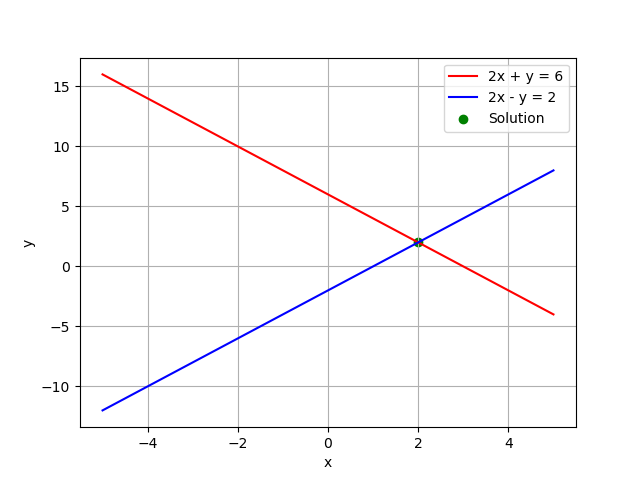
\includegraphics[width=1\columnwidth]{figs/fig.png}
        \label{stemplot}
      \end{figure}
    \end{frame}
  \end{document}
